%
%%%%%%%%%%%%%%%%%%%%%%%%%%%%%%%%%%%%%%%%%%%%%%%%%%%
%
%  S T A N D   D E R   T E C H N I K
%
%%%%%%%%%%%%%%%%%%%%%%%%%%%%%%%%%%%%%%%%%%%%%%%%%%%
\chapter{Stand der Technik}
\label{cha:technik}
%
%
Im Folgenden werden vergleichbare Arbeiten, Projekte und deren Einsatzgebiete angeführt. Es wird zunächst auf vergleichbare Projekte und anschließend auf die in der Arbeit verwendeten Technologien eingegangen. Dabei wird analysiert, warum eine Technologieanalayse im Kontext dieser Arbeit sinnvoll ist.
%
%
%
%%%%%%%%%%%%%%%%%%%%%%%%%%%%%%%%%%%%%%%%%%%%%%%%%%%
%
% A U F B A U 
%
%%%%%%%%%%%%%%%%%%%%%%%%%%%%%%%%%%%%%%%%%%%%%%%%%%%
%
\section{Bestehende Lösungsansätze}
\label{sec:vergleiche}
%
\subsection{Flyeralarm}
\label{sec:flyeralarm}
%
Auf der Internetseite \textit{Flyeralarm} gibt es nicht nur die Möglichkeit Flyer zu drucken. Es gibt sehr viele Kategorien mit einigen Produkten. Eine der Kategorien sind Becher. Man hat auch die Möglichkeit Mehrwegbecher zu bedrucken (siehe Abbildung \ref{fig:flyeralarm}).
%
\begin{figure}
	\centering
	{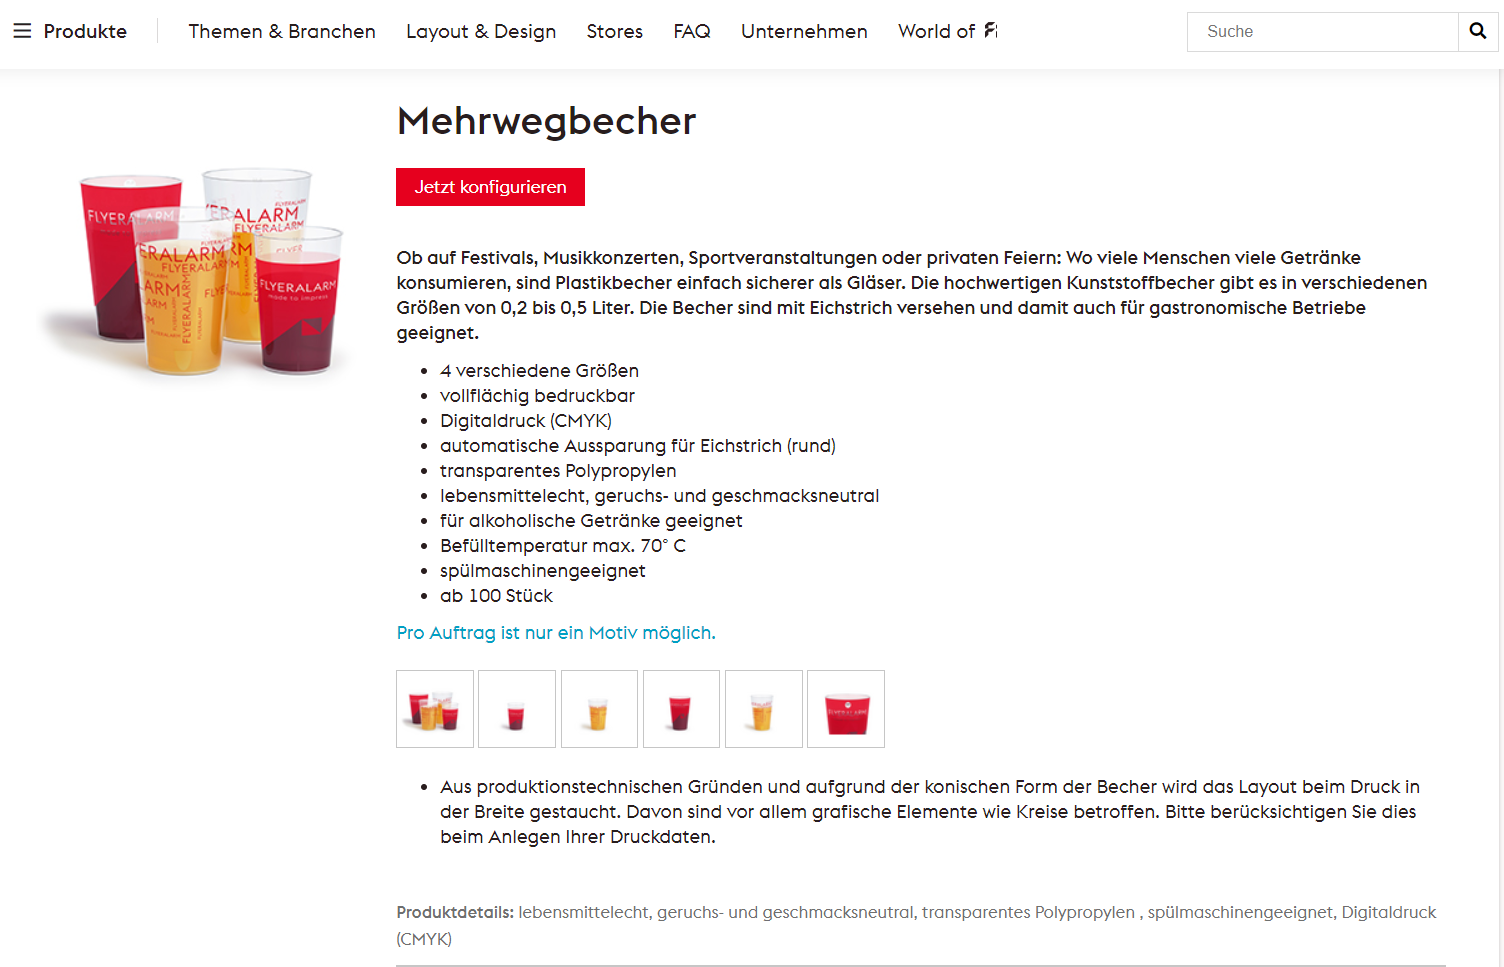
\epsfig{file = technik/images/flyeralarm.png, width=11.0cm}}
	\caption[Mehrwegbecher bestellen]{\textit{Bestellvorgang von Mehrwegbechern auf flyeralarm.com}}
	\label{fig:flyeralarm}
\end{figure}
% 
Dazu muss man, nachdem man die gewünschte Größe gewählt hat, sein Design hochladen. Dabei sollte man das Datenblatt\footnote{Das Datenblatt ist auf der Webseite zu finden und kann von dort heruntergeladen werden.} berücksichtigen, welches die Vorgaben beschreibt wie zum Beispiel Sicherheitsabstand oder Druck Farbraum. Die Online-Druckerei schreibt auf ihrer Webseite:\textit{\glqq Aus produktionstechnischen Gründen und aufgrund der konischen Form der Becher wird das Layout beim Druck in der Breite gestaucht. Davon sind vor allem grafische Elemente wie Kreise betroffen.\grqq} \cite{flyeralarm_mehrwegbecher_nodate} Eine Vorschau, wie das ganze am Ende aussehen wird, gibt es nicht. Im schlechtesten Fall hat man am Ende ein nicht zufriedenstellendes Ergebnis. Auch andere Seiten bieten ein ähnliches Angebot.Eine fertige Vorschau ist jedoch eher nicht zu finden.
%
\subsection{Spread Shirt}
\label{sec:spreadshirt}
%
Spreadshirt ist eigentlich eine Onlinedruckerei für T-Shirts. Sie selbst schreiben über sich Folgendes: \textit{\glqq Seit 2002 liefert Dir Spreadshirt T-Shirt-Druck in bester Qualität. Was als Start-up-Idee in Leipzig begann, ist inzwischen ein weltweit erfolgreiches Print-on-Demand-Unternehmen, das Wert auf faire Handels- und Produktionswege legt, seine Verantwortung als internationaler Arbeitgeber ernst nimmt und seinen Mitarbeitern ein attraktives Arbeitsumfeld bietet.\grqq } \cite{spreadshirt_tassen_nodate}
%
\begin{figure}[h]
	\centering
	{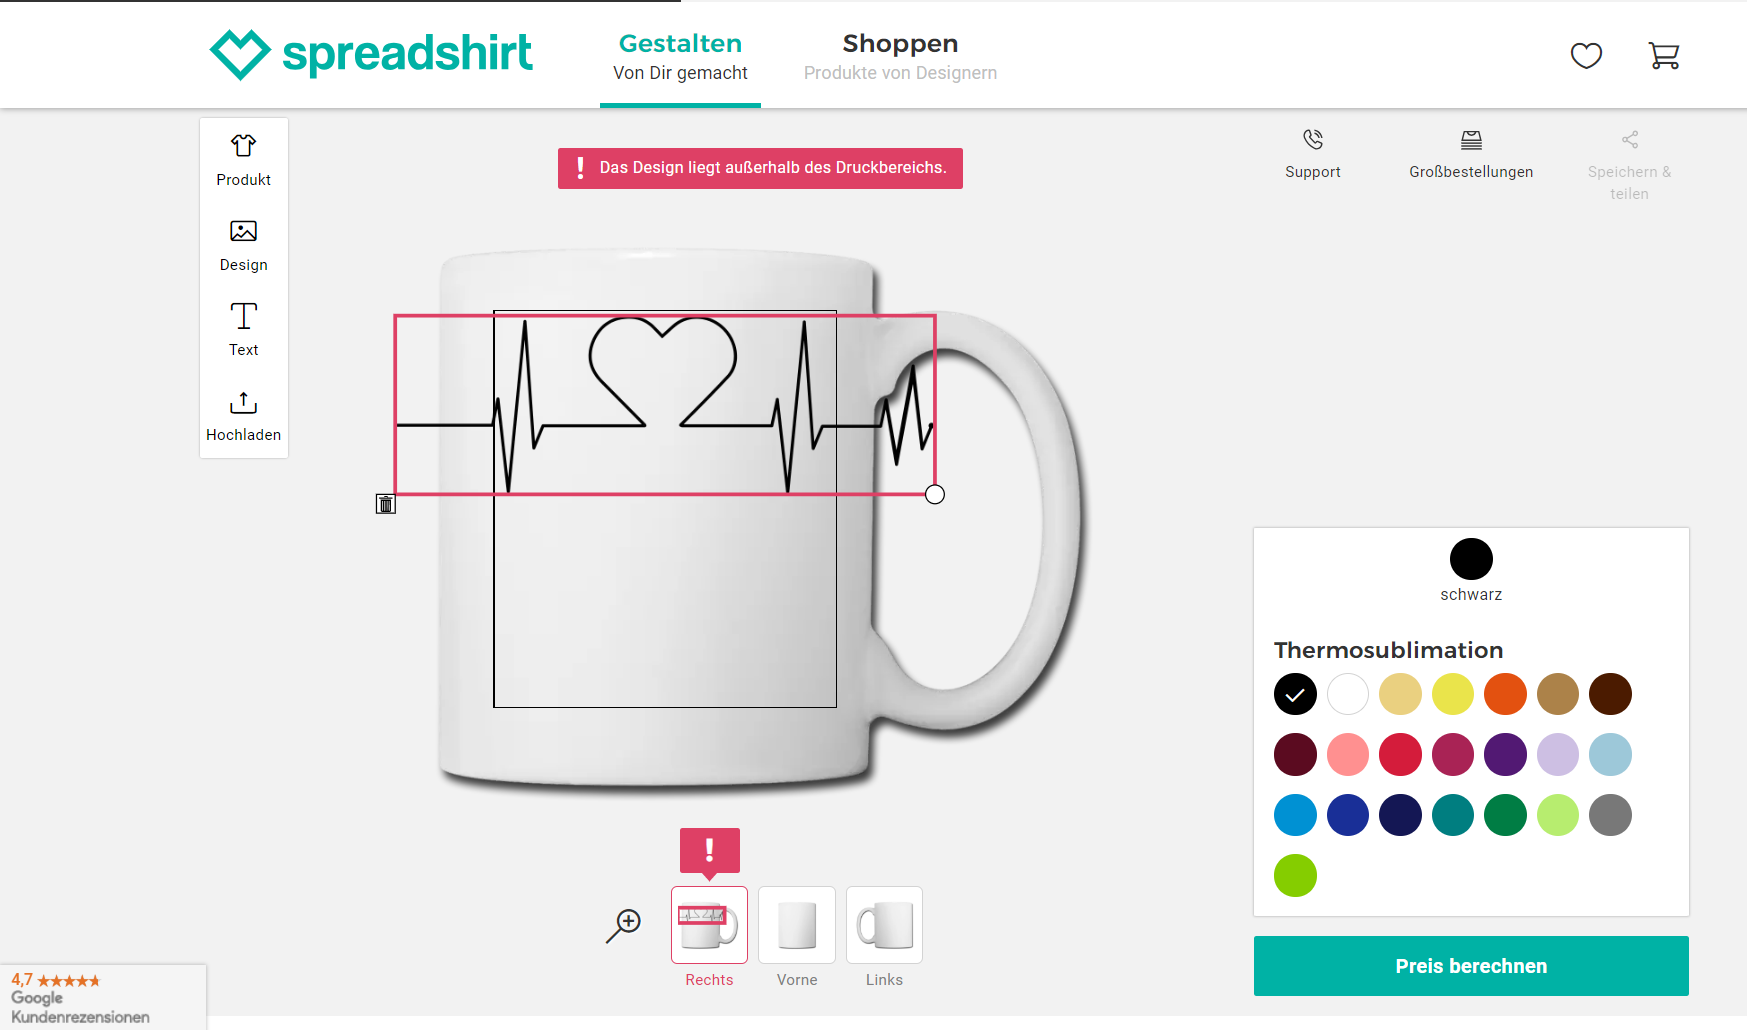
\epsfig{file = technik/images/spread-shirt.png, width=11.0cm}}
	\caption[Tasse bestellen]{\textit{Gestaltung einer Tasse auf spread-shirt.com}}
	\label{fig:spread}
\end{figure}
%
Zwar wird kein Druck von Mehrwegbechern angeboten, dafür aber der Druck von Tassen. Der Kunder kann hier in einem Online-Konfigurator seine Tasse selbst gestalten, indem er Text oder Bildelemente auf die Tasse legt. Das ganze wird sogar in 3D angezeigt. Jedoch ist die Ansicht nicht flexibel sondern statisch. Man kann die Tasse lediglich von drei verschiedenen Blickwinkeln betrachten (rechts, vorne, links). In unserem Fall sollen fertige Designs dargestellt werden. Auch das ist beim Tassenkonfigurator von Spreadshirt schwierig. Wie in der Abbildung \ref{fig:spread} zu sehen kann ein Objekt nur im Druckbereich dargestellt werden, nicht außerhalb des Bereichs. Damit ist ein Rundum-Druck nicht möglich. \\
Trotzdem lässt sich sagen, dass dieser Konfigurator gut und übersichtlich gestaltet ist. Jedoch hat er nicht die Funktionalität, welche der Konfigurator für Gizeh haben sollte.
%
\subsection{Becher-bedrucken.de}
\label{sec:currycup}
%
Ein weiteres Angebot für Becher gibt es auf \textit{becher-bedrucken.de}. Dort gibt es einen 3D Konfigurator für verschiedene Becher. Der technische Ansatz ist schon sehr gut und kann bei der Entwicklung berücksichtigt werden. Es werden ähnliche Technologien verwendet, wie in dieser Arbeit. Jedoch sind die Designvorgaben ganz anders als die Druckvorgaben von Gizeh. Das hochgeladene Design ist so angepasst, das es bestmöglich auf dem Becher angezeigt werden kann.
%
\begin{figure}[h]
	\centering
	{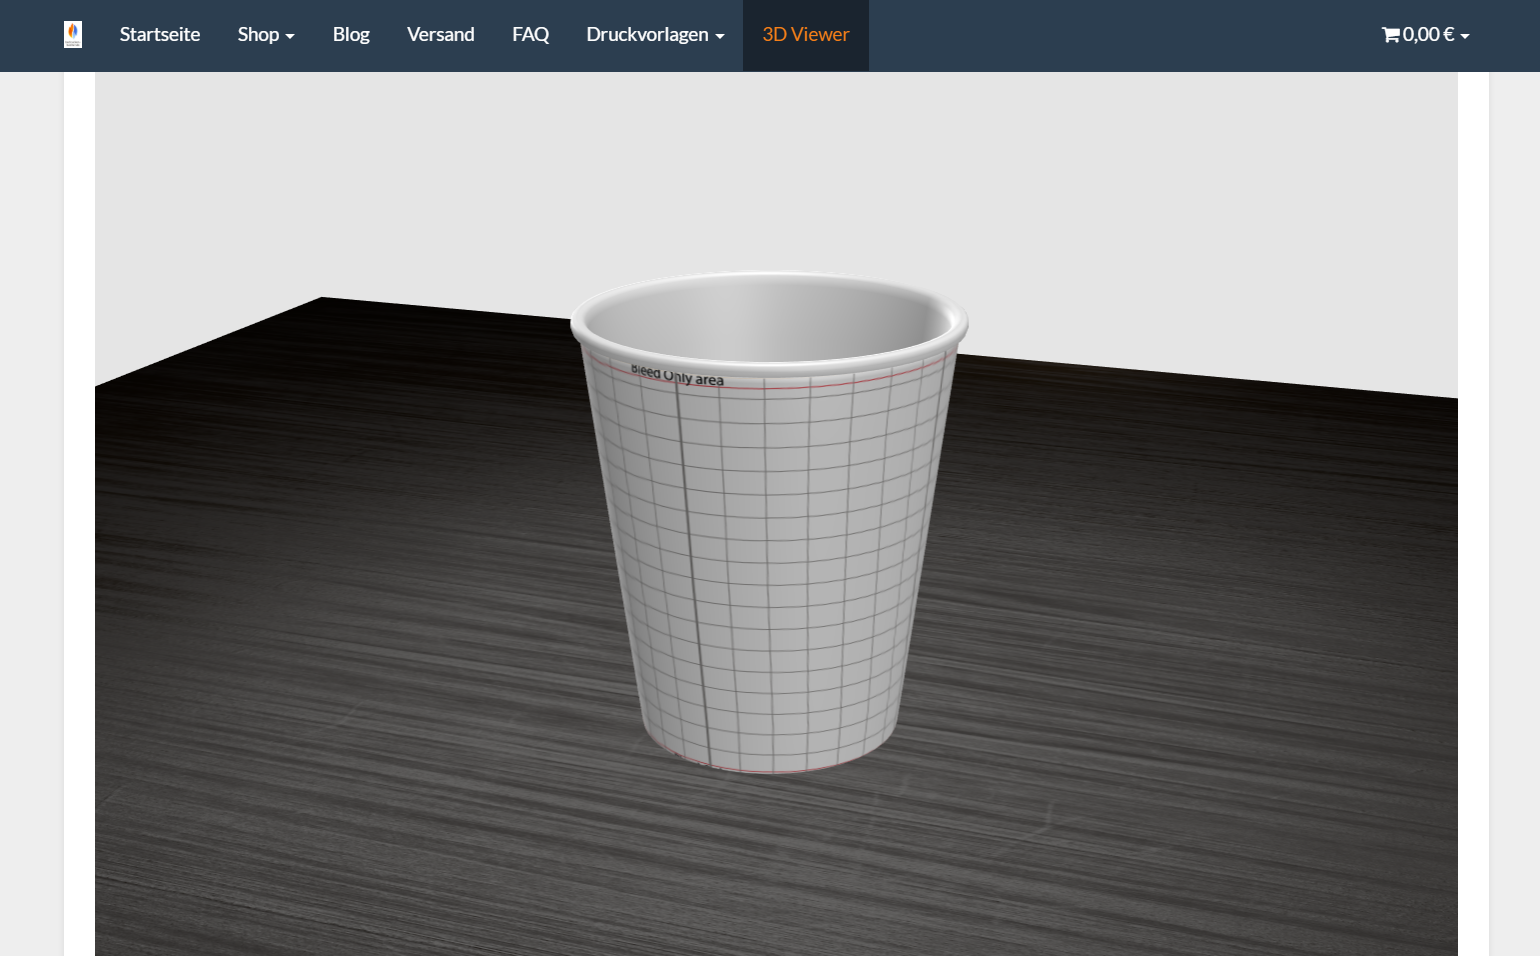
\epsfig{file = technik/images/becher-bedrucken.png, width=11.0cm}}
	\caption[Becher bedrucken]{\textit{3D Viewer eines Bechers auf bedrucken-becher.de}}
	\label{fig:becherbedrucken}
\end{figure}
%
Die Darstellung in 3D ist schön anzusehen. Zumindest auf einem Gerät mit größerem Display. Eine Anpassung für mobile Geräte ist so gut wie gar nicht vorhanden. Technisch gesehen kann aber trotzdem an diesen Lösungsansatz angeknüpft werden.
%
\section{3D Online Konfiguratoren}
\label{sec:3dconfigurators}
%
Heutzutage kann nahezu alles bedruckt werden. Die Vielzahl an Produkten ist groß. Dies haben wir bisher in diesem Kapitel erläutert, wie das konkret bei Bechern oder Tassen aussehen kann. Schwieriger zu finden sind allerdings 3D Konfiguratoren für diese Produkte. Oft gibt es höchsten eine 3D Pop-Up Ansicht, eine alte Lösung mit Flash o. ä. Eine responsive Lösung ist eher nicht zu finden. \\
In der Autoindustrie und anderen Branchen sind jedoch einige gute 3D Konfiguratoren umgesetzt. Wenn man eventuell die passenden Felgen sucht, bekommt man da einen übersichtlich gut gestalteten Konfigurator in 3D. Teilweise sind Konfiguratoren zu finden, welche responsiv sind. Einige Firmen bieten sogar an 3D Konfiguratoren für bestimmte Produkte umzusetzen. Dabei handelt es sich meist um individuelle Lösungen. Das Folgende Beispiel soll zeigen, das es durchaus möglich ist gute 3D Konfiguratoren zu entwickeln.
%
\begin{figure}[]
	\centering
	{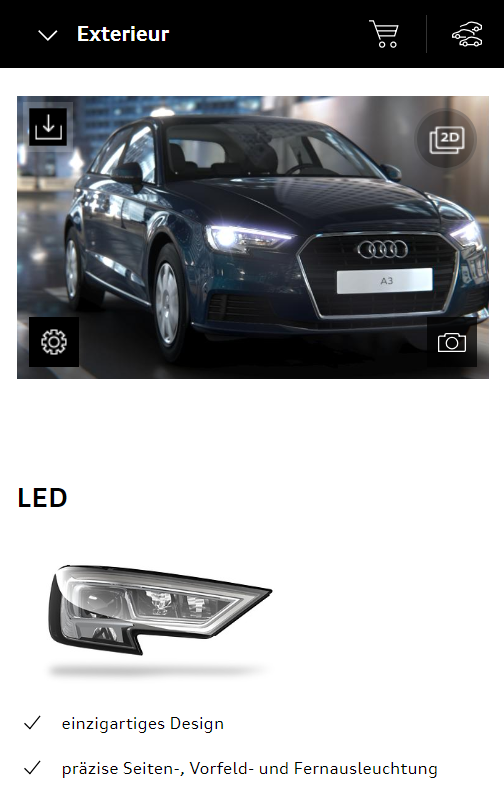
\epsfig{file = technik/images/audi.png, width=6.0cm}}
	\caption[Audi Konfigurator]{\textit{Neue 3D Ansicht von Audi}}
	\label{fig:audi}
\end{figure}
%
%
\paragraph{Audi 3D Konfigurator}Letztes Jahr veröffentlichte Audi seinen neuen Konfigurator auf der Webseite. Er rendert die Fahrzeuge in Echtzeit. Die Anwendung ist auch für mobile Geräte optimiert (siehe Abbildung \ref{fig:audi}). So kann man den Konfigurator beispielsweise mit Toucheingaben steuern. Man kann sich das Fahrzeug ganz genau anschauen und an Details heranzoomen. Technisch eine sehr gute Umsetzung, die auch optisch etwas her macht. Für die Zukunft plant Audi sogar eine 4k-Darstellung. Dardurch bekommt der Benutzer eine noch realistischere Ansicht des Wagens. \\
%
%
\paragraph{Siemens 3D Konfigurator}Immer mehr Firmen präsentieren neue 3D Konfiguratoren für ihre Produkte. So auch 2018 Siemens. Mit einem 3D Konfigurator ist es nun möglich Systemschaltschränke am 3D-Modell zu konfigurieren. Dabei wählt der Nutzer die verschiedenen Module, welche in den Schaltschrank verbaut werden sollen, in mehreren Schritten aus. Der Konfigurator prüft dabei, ob eine Kombination der Module möglich ist. Sogar eine Exportfunktion für CAD-Programme ist in den Konfigurator integriert. Die Kosten der Zusammenstellung werden auch in einer übersicht dargestellt.\\
%
\begin{figure}[]
	\centering
	{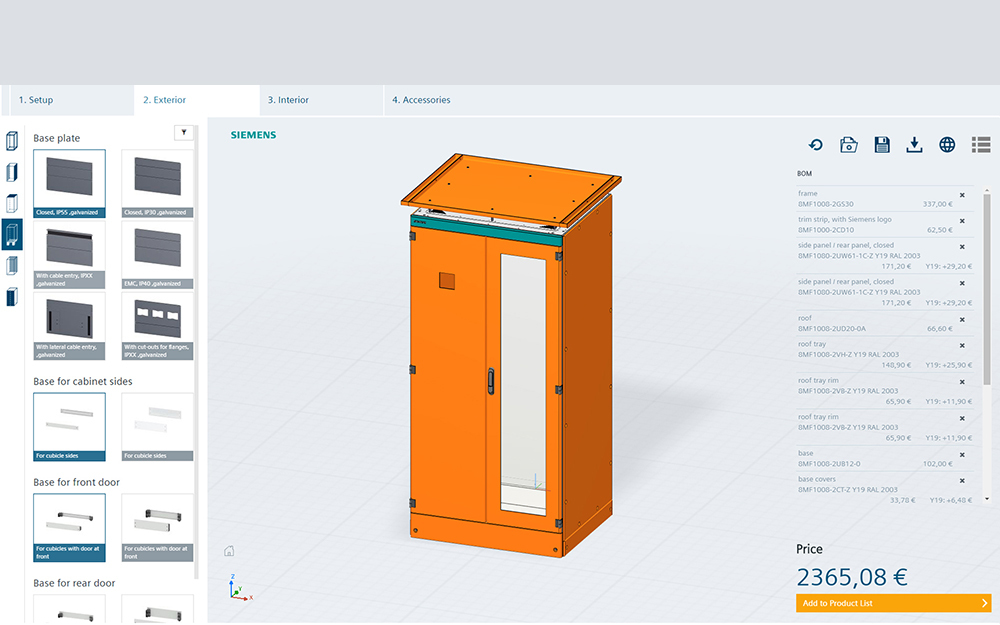
\epsfig{file = technik/images/siemens.png, width=13.0cm}}
	\caption[Audi Konfigurator]{\textit{Neuer 3D Konfigurator von Siemens für Systemschaltschränke}}
	\label{fig:siemens}
\end{figure}
%
\paragraph{Trilux Limba 3D Konfigurator} TRILUX Symplify Your Light steht für den einfachsten und sichersten Weg zu einer maßgeschneiderten, energieeffizienten und zukunftsfähigen Lichtlösung. Das Unternehmen hat auf seiner Webseite zu verschiedenen Produkten einen Konfigurator. Es ist eine einfache und schnelle Hilfe bei der Suche nach der richtigen Beleuchtung. Dabei ist es möglich, das Produkt nach belieben anzupassen und zu konfigurieren. Am Ende lässt sich das ganze in einer PDF exportieren. Das hilft dem Kunden enorm, da er sich das Produkt besser vorstellen kann und es leichter fällt eine Entscheidung bezüglich der Auswahl zu treffen.\\
%
\section{Webframeworks}
\label{sec:webframeworks}
%
Heutzutage werden Frameworks wie \textit{Angular} oder \textit{ReactJS} verwendet um performante und benutzerfreundliche Webanwendungen zu entwickeln. Es handelt sich dabei um JavaScript-Frontend-Frameworks. Man hat oft die Qual der Wahl, da in den letzten Jahren einige Frameworks entwickelt bzw. weiterentwickelt wurden. Die Anzahl der Angebote an JavaScript-Frameworks und -Libraries ist groß. Sie kommen oft beim Entwickeln von \textit{Single Page Applications (SPA)}\footnote{Was Single Page Anwendungen sind wird im Kapitel Grundlagen genauer beschrieben.}  zum Einsatz.
%
\paragraph{Angular}
\label{p:angular}
%
ist nichts anderes als ein JavaScript-Framework auf Basis von TypeScript\footnote{Eine von Microsoft entwickelte Programmiersprache. TypeScript ist eine kompilierte und plattformübergreifende Sprache, die reine JavaScript-Dateien generiert.}. Es wurde von Google entwickelt und ist ein Open-Source-Framework. Es unterstützt den Entwickler dabei, moderne Webanwendungen zu machen, die zum einen für Desktop und zum andern für Mobile optimiert worden sind. Wie in der Abbildung \ref{fig:googletrends} zu sehen, ist \textit{Angular} das meist genutzte und bekannteste Framework für SPAs. Ähnliches zeigt auch die Stack Overflow Entwicklerumfrage 2018: Bei den meist genutzen Bibliotheken und Frameworks liegt Angular mit 36,9\% einen Platz vor React mit 27,8\% \cite{stackoverflow_stack_2018}.
%
\begin{figure}[h]
	\centering
	{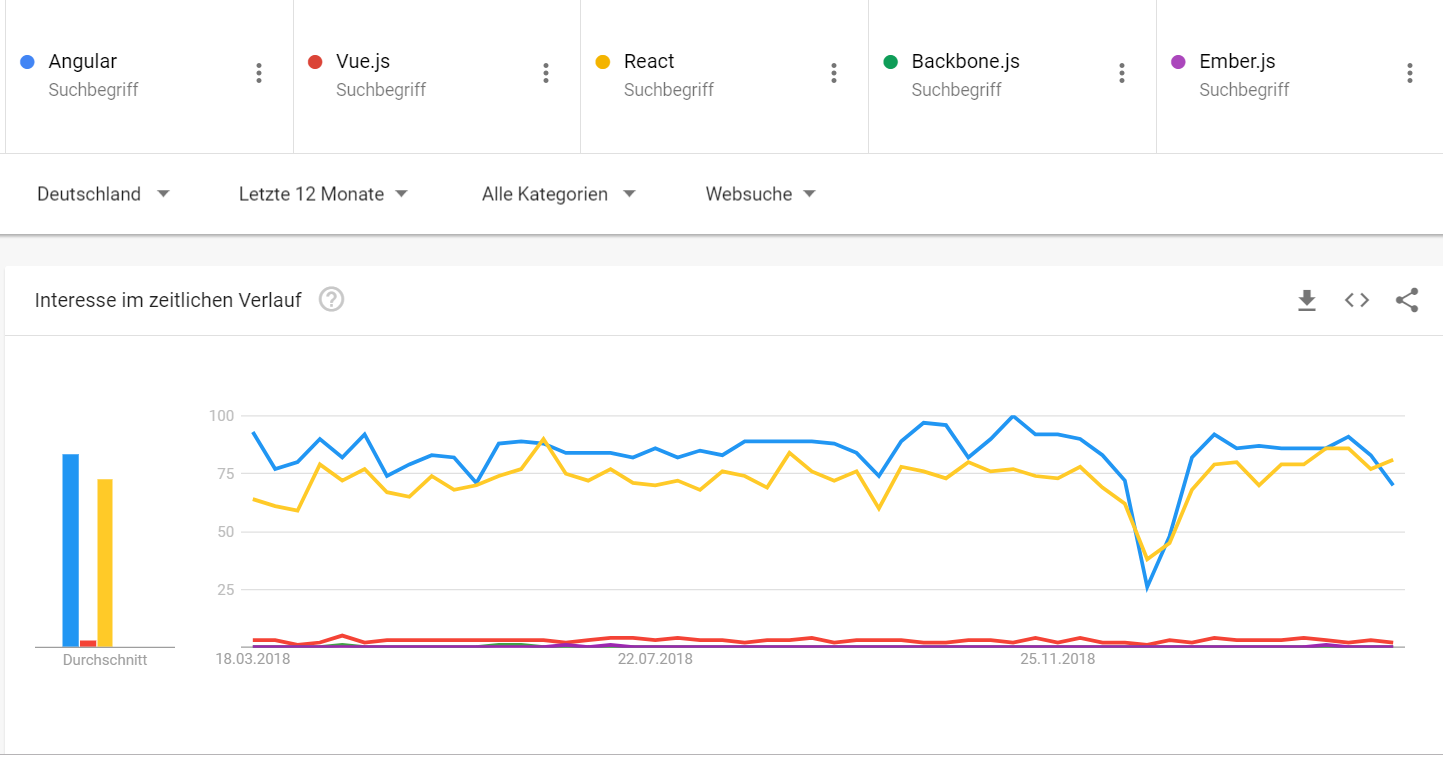
\epsfig{file = technik/images/google-trends.png, width=13.0cm}}
	\caption[Audi Konfigurator]{\textit{Google Trends Statistik. Suchanfragen von Frontend-Frameworks in 2018}}
	\label{fig:googletrends}
\end{figure}
%
Außerdem gibt es den Entwicklern Konventionen und Richtlinen an die Hand. Das ist gerade dann sinnvoll, wenn man in einem großen Team arbeitet. Oder bei großen Projekten für ein einfaches Handling und die Wartbarkeit des Codes sinnvoll wird. Ein Merkmal von Angular ist, das es viele unterschiedliche Module gibt, die es ermöglichen, sehr effizient Anwendungen zu produzieren. Das Framework ist auch bekannt für seine tollen Animationen auf Basis von Web-Animation. Ein weiteres, wichtiges Modul ist das Routing-Modul. Im Grunde genommen sind Routings Grundbestandteil für \textit{Single Page Anwendungen}. Mittels Routings kann ich festlegen welcher Teil der Anwendung nun angezeigt werden soll. Außerdem baut das Framework auf die komponentenbasierte Programmierung. In Kapitel 3 werden wir noch genauer auf Angular eingehen\footnote{Die Dokumentation des Frameworks ist unter \textit{https:/angular.io/docs/} zu finden.}.
%

%
\paragraph{React}
\label{p:react}
%
ist das meistgesuchte JavaScript Framework 2018 \cite{stackoverflow_stack_2018}. Es wurde 2013 von Facebook entwickelt und viele bekannte Unternehmen wie Netflix, Twitter oder PayPal verwenden das Framework. Ähnlich wie Angular setzt React auf modulare Komponentenarchitektur. Damit wird der Frontendcode leicht nachvollziehbar. \textit{\glqq Das Ziel von React ist es, einfacheren Code schreiben zu können, dessen Bestandteile weniger miteinander verschränkt oder verwoben sind \grqq}\cite{kogel_paul_react_2015} \\
React ist kein Framework, es ist eine Bibliothek. Es ist ein sehr flexibles Werkzeug, dass in bestehende Anwendungen eingebaut werden kann, ohne den ganzen Code umzustrukturieren. Dem Entwickler wird keine Grundstruktur für seine Applikation gegeben, was ein wesentlicher Unterschied zu Angular ist. Ein weiteres Merkmal von React ist die virtuelle DOM. Diese garantiert die Synchronisierung der DOM indem bei Änderungen alles neu gerendert wird\footnote{Die vollständige Dokumentation ist unter \textit{https://reactjs.org/docs/getting-started.html} zu finden}.
%
\paragraph{Vue.js}
\label{p:vueJS}
%
ist ein weiteres Frontend-Framework zur Entwicklung von \textit{Single Page Anwendungen}. Es ist nicht das beliebteste Framework und trotzdem taucht es immer wieder auf (siehe Abbildung \ref{fig:googletrends}) und ist definitiv eine Alternative zu \textit{Angular} oder \textit{React}. Es setzt auch auf eine modulare Architektur, die in einzelne Komponenten zerteilt ist. Das Framework ist im Vergleich zu seinen Konkurrenten deutlich einfacher und hat eine flache Lernkurve. Dadurch ist es auch schneller und bringt dem Framework einen Vorteil gegenüber den Alternativen. Obwohl es kleiner ist, bringt es trotzdem alle wichtigen Funktionen wie Suchmaschinenoptimierung mit sich. Es kann auch in Kombination mit React verwendet werden. In Vue.js wird ohnehin das bekannte virtul DOM genutzt. Auch die Community ist stetig am wachsen.\footnote{Weitere Informationen sind in der offizielen Dokumentation unter \emph{https://vue.js.org/v2/guide} zu finden.} \\
%
%
%
%%%%%%%%%%%%%%%%%%%%%%%%%%%%%%%%%%%%%%%%%%%%%%%%%%%
%
% A U F B A U 
%
%%%%%%%%%%%%%%%%%%%%%%%%%%%%%%%%%%%%%%%%%%%%%%%%%%%
%
\section{Flash und WebGL}
\label{sec:webgl2}
%
In dem Artikel \emph{HTML5/WebGL vs Flash in 3D Visualisation} schreibt der Autor folgendes über WebGL:\\

\textit{\glqq The development of improved 3D graphics in Web-based applications took a step forward recently, when programmers began building WebGL into the Mozilla Firefox nightly builds, and into WebKit, which is used by Google Chrome and Apple's Safari browser. WebGL is one of the most developed libraries which are supported by HTML5.\grqq } \cite{bahor_html5/webgl_2013}.\\

Adobe Flash ist auch heute noch vielen ein Begriff. Es war darauf ausgerichtet interaktive 2D Grafiken im Web bereitzustellen. Mit der Veröffentlichung der Version 10 des Flash Players haben die Entwickler sogar eine z-Achse eingeführt. Sie ermöglicht eine 3D Darstellung und Transformation von Objekten. Diese Unterstützung für die Interaktion von Objekten der dritten Dimension wurde jedoch in begrenzter Weise bereitgestellt.\\
Einer der aktuellsten Leistungstests zwischen dem Flash- und dem WebGL-Canvas-basierten 3D-Inhalt zeigt deutlich, dass der HTML5-Canvas beginnt, höhere Frameraten zu generieren und 3D-Inhalte im Web zu rendern. Die Testergebnisse zeigen, dass WebGL beim Rendern von 3D-Inhalten wesentlich schneller abschneidet und höhere Frameraten für die 3D-Animationen im Web bietet, während sie mit Flash verglichen werden. Weiter schreibt Senad Bahor in seinem Artikel: \textit{\glqq And actually, that ist what the 3D graphics is all about, about altering the 3D model abd see it change on time basis. This is something that can currently be achieved only with the usage of the HTML5 and WebGL engines on the web [...] \grqq} \cite{bahor_html5/webgl_2013} 3D-Modelle zu ändern und sie zu animieren kann also derzeit nur durch die Verwendung von HTML5 und WebGL im Web erreicht werden.\\
Weiter zeigen die Ergebnisse des Artikels deutlich, dass Flash-basierte 3D-Grafiken auf iOS-basierten Geräten nahezu nicht darstellbar sind, da Adobe mit seinem Flash-Plugin nie iOS unterstützt hat. Aufgrund der HTML5-Funktionalität und -Erreichbarkeit kann die Webseite auch auf einer Vielzahl von Geräten, einschließlich iOS- und Android-Geräten, wiedergegeben werden, ohne dass sich die Benutzer um das Vorhandensein der Plugins und die Versionierung des Players kümmern müssen.
Webbrowser entwickeln sich stetig weiter. WebGL kann in über 95\% aller Browser verwendet werden \cite{deveria_alexis_can_2013}. Was zuvor schon in Videopielen mit OpenGL möglich war, ist nun auch im Web möglich. Wie genau WebGL als Abstraktionsschicht für den grafischen Teil einer Anwendung verwendet werden kann, wird in Kapitel \ref{sec:javascriptbibliotheken} erläutert.

Mit WebGL müssen die Benutzer nicht dazu aufgefordert werden, eines der Plugins zu installieren, um den 3D-Inhalt auf der Website zum Laufen zu bringen. Die einzige Voraussetzung ist, dass der Webbrowser das HTML5-Canvas-Element unterstützt, über das WebGL den Inhalt für den Benutzer darstellt.\\
Im Wesentlichen kann WebGL auf jeder Plattform und auf allen großen Systemen mit OpenGL-fähiger Grafikkarte und einem Browser ausgeführt werden, der WebGL unterstützt.\\

\section{3D JavaScript Bibliotheken}
\label{sec:javascriptbibliotheken}
%
Um eine 3D Szene mit WebGL darzustellen wird ein JavaScript Framework benötigt. Es erstellt und rendert eine Szene mit den 3D Objekten. Im Folgenden werden die zwei bekanntesten und weit verbreitetsten Bibliotheken vorgestellt.
\paragraph{ThreeJS}
\label{sec:threeJS}
%
\textit{Three.js} ist es eine sehr seriöse WebGL-Bibliothek mit einer starken Community und vielen guten Beispielen. Es wird auch oft in kommerziellen Webanwendungen verwendet. Die erste Version des Frameworks tauchte 2010 auf und der Quellcode wird in einem Repository auf GitHub gehostet\footnote{https://github.com/mrdoob/three.js/}. Three.js hat eine verständliche Struktur und große Anpassungsmöglichkeiten. Es ist eine Anwendungsprogrammierschnittstelle, mit der animierte 3D-Grafiken in einem Webbrowser erstellt und angezeigt werden. Neben der Dokumentation gibt es auch ein Wiki, was dem Entwickler zum schnellen Einstieg sehr helfen kann\footnote{https://github.com/mrdoob/Three.js/wiki/}.Schon beim erstellen einer einfachen Szene mit dem Framework fällt auf, das es dem Prinzip der objektorientierten Programmierung folgt\footnote{https://threejs.org/docs/\#manual/en/introduction/Creating-a-scene}. In dem Kapitel \ref{cha:introduction} wird noch genauer auf das Framework eingegangen.
%
%\begin{figure}[h]
%	\centering
%	{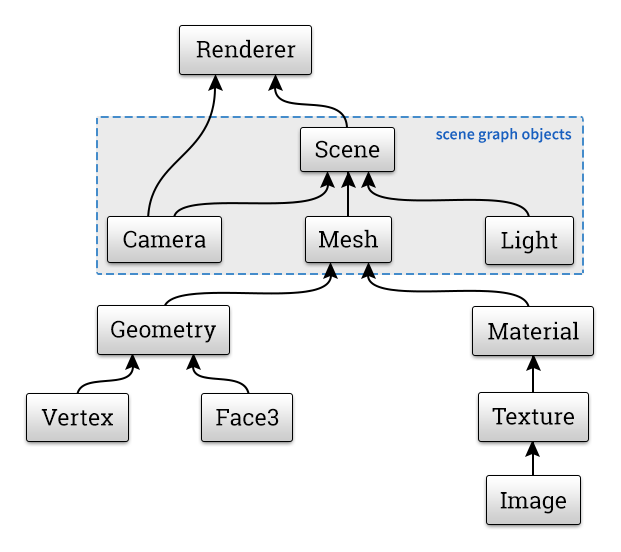
\epsfig{file = technik/images/node-map.png, width=11.0cm}}
%	\caption[Audi Konfigurator]{\textit{Aufbau einer Szene in Three.js}}
%	\label{fig:threejs}
%\end{figure}
%
%
\paragraph{BabylonJS}
\label{sec:babylonJS}
%
Babylon.js\footnote{Die offizielle Dokumentation ist unter \textit{https://doc.babylonjs.com/} zu finden.} ist ein Framework, mit dem komplette 3D-Webanwendungen erstellen werden können. Babylon.js hat eine Community, die stetig wächst und auch aktiv zum Projekt beiträgt und immer mehr Funktionen hinzufügt. Das Framework hat alle notwendigen Werkzeuge, um 3D-Anwendungen umzusetzen. Sie können 3D-Objekte laden und zeichnen, diese 3D-Objekte verwalten, Spezialeffekte erstellen und verwalten, räumliche Sounds spielen und verwalten, Gameplay erstellen und vieles mehr. 
%
\begin{figure}[h]
	\centering
	{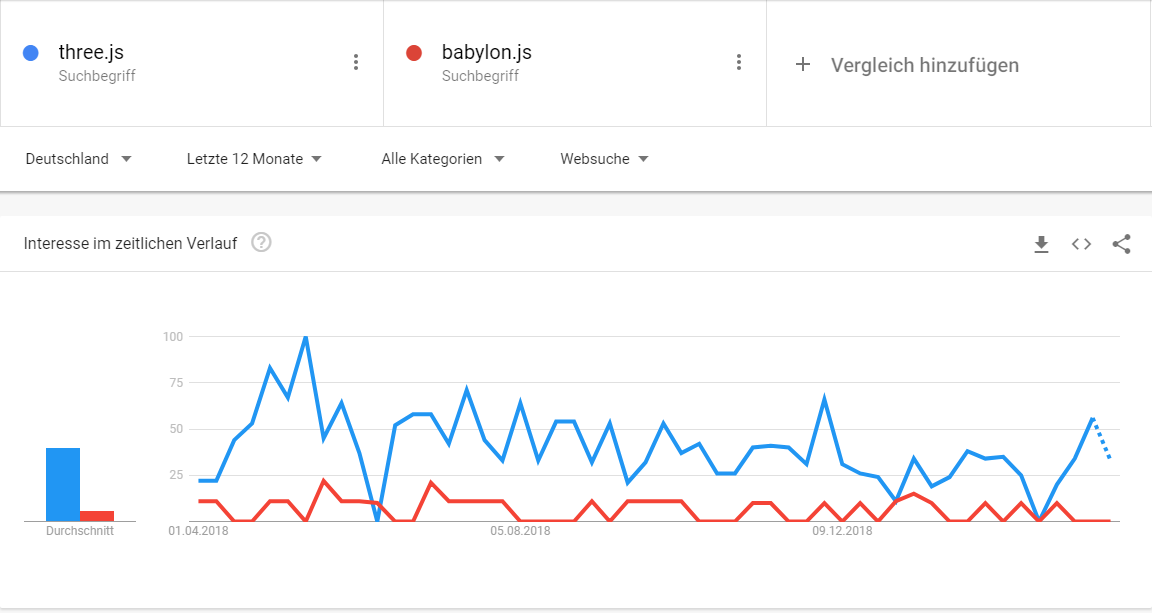
\epsfig{file = technik/images/3d-framework.png, width=13.0cm}}
	\caption[Audi Konfigurator]{\textit{Google Trends: Vergleich Three.js und Babylon.js in den letzten 12 Montaten}}
	\label{fig:compare3dframework}
\end{figure}
%
Babylons.js ist ein benutzerfreundliches Framework, da Sie diese Dinge mit den minimalen Codezeilen einrichten können. Es ist ein mit TypeScript entwickeltes JavaScript-Framework. (vgl. \cite{moreau-mathis_babylon.js_2016}) Wie in Abbildung \ref{fig:compare3dframework} zu sehen ist Babylon.js jedoch weniger gefragt als three.js. Das zeigt sich auch in den 3D Webanwendungen, wo auch meist three.js verwendet wird.
